\documentclass{article}

% if you need to pass options to natbib, use, e.g.:
%     \PassOptionsToPackage{numbers, compress}{natbib}
% before loading neurips_2019

% ready for submission
 \usepackage{neurips_2019, times}
% to compile a preprint version, e.g., for submission to arXiv, add add the
% [preprint] option:
     %\usepackage[preprint]{neurips_2019}

% to compile a camera-ready version, add the [final] option, e.g.:
%   \usepackage[final]{neurips_2019}

% to avoid loading the natbib package, add option nonatbib:
%     \usepackage[nonatbib]{neurips_2019}

\usepackage[utf8]{inputenc} % allow utf-8 input
\usepackage[T1]{fontenc}    % use 8-bit T1 fonts
\usepackage{hyperref}       % hyperlinks
\usepackage{url}            % simple URL typesetting
\usepackage{booktabs}       % professional-quality tables
\usepackage{amsfonts}       % blackboard math symbols
\usepackage{nicefrac}       % compact symbols for 1/2, etc.
\usepackage{microtype}      % microtypography
\usepackage{graphicx}

\usepackage{geometry}
\usepackage{amsmath}
\usepackage{cancel}

\newcommand{\bM}{\mathbf{M}}
\newcommand{\bv}{\mathbf{v}}
%\newcommand{\be}{\mathbf{e}}
\newcommand{\bI}{\mathbf{I}}

\title{PCA Normalization}

% The \author macro works with any number of authors. There are two commands
% used to separate the names and addresses of multiple authors: \And and \AND.
%
% Using \And between authors leaves it to LaTeX to determine where to break the
% lines. Using \AND forces a line break at that point. So, if LaTeX puts 3 of 4
% authors names on the first line, and the last on the second line, try using
% \AND instead of \And before the third author name.

\author{%
  David S.~Hippocampus\thanks{Use footnote for providing further information
    about author (webpage, alternative address)---\emph{not} for acknowledging
    funding agencies.} \\
  Department of Computer Science\\
  Cranberry-Lemon University\\
  Pittsburgh, PA 15213 \\
  \texttt{hippo@cs.cranberry-lemon.edu} \\
  % examples of more authors
  % \And
  % Coauthor \\
  % Affiliation \\
  % Address \\
  % \texttt{email} \\
  % \AND
  % Coauthor \\
  % Affiliation \\
  % Address \\
  % \texttt{email} \\
  % \And
  % Coauthor \\
  % Affiliation \\
  % Address \\
  % \texttt{email} \\
  % \And
  % Coauthor \\
  % Affiliation \\
  % Address \\
  % \texttt{email} \\
}

\begin{document}

\maketitle

\begin{abstract}

\end{abstract}

\section{Experiment}

%\begin{table}[!htb]
%\begin{centering}
%\begin{tabular}{|c|c|c|c|}
%\hline
%Norm Methods          & BN        & PCA       & ZCA       \\ \hline
%Power Iteration No.   & -         & 20        & 20        \\ \hline
%Initial Eng-Vector    & -         & Identity  & Identity  \\ \hline
%Minimum Error         & 5.39      & 4.88      & 5.38      \\ \hline
%Mean Error (4 trials) & 5.66-0.28 & 5.57-0.46 & 5.52-0.15 \\ \hline
%\end{tabular}
%\caption{CIFAR-10 test errors.}
%\end{centering}
%\end{table}

\section{PCA Norm Layer}
Options to implement PCA Norm Layer.
\begin{itemize}
\item Given input covariance matrix $\bM$, use \textbf{Eigen Decomposition} or \textbf{Singular Value Decomposition (SVD)} Operation as forward computation, and use the analytic solution of its gradient for backward propogation.
\item Given input covariance matrix $\bM$, vectors with random values $[\bv_1^{1}, \bv_2^{1}, ...]$, use \textbf{Power Iteration} as forward computation, and use its gradient for backward propogation.
\item Given input covariance matrix $\bM$, vectors with random values $[\bv_1^{1}, \bv_2^{1}, ...]$, use \textbf{Eigen Decomposition} or \textbf{SVD} Operation as forward computation, and use \textbf{Power Iteration} to approximate the analytic solutions of the gradient for backward propogation.
\end{itemize}

Usually, people choose either option 1 or option 2 to implement PCA Norm Layer, but both of them have problems.
In option 1, \textbf{Eigen Decomposition} or \textbf{Singular Value Decomposition (SVD)}, the analytic solutions of the gradient sometimes causes NaN problem when there are two or more eigenvalues are too close to each other.
In option 2, if the two eigenvalues are very close, eigenvectors could not be computed precisely with limited power iteration number. Thus, during backprorogation, the derivatives will be very inaccurate and destroy the parameters of model, and cause numerical instability in the training process.

In this paper, we propose to using option 3. During forward pass, we use \textbf{SVD} to compute the eigenvalues. 
SVD is numerically more stable than eigendecomposition \cite{nakatsukasa2013stable} as SVD implementation employs a divide-and-conquer strategy, while the eigendecomposition uses QR algorithm. 
During backpropogation, we employ \textbf{Power Iteration} method to compute the numerical solutions of the covariance matrix $\bM$ gradient.
In \textbf{sections} \ref{sec: pi} \& \ref{sec: mbp}, we will prove that when the iteration number goes to infinite, the accumulated gradients (\emph{i.e.} numerical solution) from the \textbf{Power Iteration} method is exactly the same with the analytic solution of the gradient.


\newpage

\section{Approximate SVD gradient with Power Iteration in backpropogation}
In the following 2 subsections, we will prove that when the gradient computed from Power Iteration equals to the gradients computed from SVD.
	\subsection{Power Iteration}
	\label{sec: pi}
	The following gradient formula for power iteration methods is from~\cite{ye2017dynamic}.
	\begin{equation}
	\begin{aligned} 
	\frac{\partial L}{\partial \bM} &=\sum_{k} \frac{\left(\bI-\bv^{(k+1)} \bv^{(k+1)\top}\right)}{\left\|\bM \bv^{(k)}\right\|} \frac{\partial L}{\partial \bv^{(k+1)}} \bv^{(k)\top} \\
	\frac{\partial L}{\partial \bv^{(k)}} &=\bM \frac{\left(\bI-\bv^{(k+1)} \bv^{(k+1)\top}\right)}{\left\|\bM \bv^{(k)}\right\|} \frac{\partial L}{\partial \bv^{(k+1)}} 
	\end{aligned}
	\end{equation}
	Using 3 power iteration steps for demonstration.
	\begin{equation}
	\begin{aligned} 
	\frac{\partial L}{\partial \bv^{(2)}} &=\bM \frac{\left(\bI-\bv^{(3)} \bv^{(3)\top}\right)}{\left\|\bM \bv^{(2)}\right\|} \frac{\partial L}{\partial \bv^{(3)}}\\
	\frac{\partial L}{\partial \bv^{(1)}} &=\bM \frac{\left(\bI-\bv^{(2)} \bv^{(2)\top}\right)}{\left\|\bM \bv^{(1)}\right\|} \frac{\partial L}{\partial \bv^{(2)}}\\
	&=\bM \frac{\left(\bI-\bv^{(2)} \bv^{(2)\top}\right)}{\left\|\bM \bv^{(1)}\right\|} 
	\bM \frac{\left(\bI-\bv^{(3)} \bv^{(3)\top}\right)}{\left\|\bM \bv^{(2)}\right\|} \frac{\partial L}{\partial \bv^{(3)}}
	\end{aligned}
	\end{equation}
	
	Then the $\frac{\partial L}{\partial \bM}$ should be like the following, for the reason that we use eigenvalue decomposition (ED)'s result as initial value, then $\bv^{(0)}\approx\bv^{(1)}\approx\bv^{(2)}$. We use $\bv$ to represent it, M is symmetric.
	
	\begin{equation}
	\begin{aligned} 
	\frac{\partial L}{\partial \bM}
	&=\frac{\left(\bI-\bv^{(3)} \bv^{(3)\top}\right)}{\left\|\bM \bv^{(2)}\right\|} \frac{\partial L}{\partial \bv^{(3)}} \bv^{(2)\top} +
	\frac{\left(\bI-\bv^{(2)} \bv^{(2)\top}\right)}{\left\|\bM \bv^{(1)}\right\|} \frac{\partial L}{\partial \bv^{2}} \bv^{(1)\top} + 
	\frac{\left(\bI-\bv^{(1)} \bv^{(1)\top}\right)}{\left\|\bM \bv^{(0)}\right\|} \frac{\partial L}{\partial \bv^{(1)}} \bv^{(0)\top}\\
	&=\frac{\left(\bI-\bv \bv^{\top}\right)}{\left\|\bM \bv\right\|}\left(\frac{\partial L}{\partial \bv^{(3)}} + \frac{\partial L}{\partial \bv^{(2)}} + \frac{\partial L}{\partial \bv^{(1)}} \right)\bv^{\top}\\
	&=\frac{\left(\bI-\bv \bv^{\top}\right)}{\left\|\bM \bv\right\|}\left(\frac{\partial L}{\partial \bv^{(3)}} +
	\bM \frac{\left(\bI-\bv \bv^{\top}\right)}{\left\|\bM \bv\right\|} \frac{\partial L}{\partial \bv^{(3)}} + 
	\bM \frac{\left(\bI-\bv \bv^{\top}\right)}{\left\|\bM \bv\right\|} 
	\bM \frac{\left(\bI-\bv \bv^{\top}\right)}{\left\|\bM \bv\right\|} \frac{\partial L}{\partial \bv^{(3)}}
	\right)\bv^{\top}\\
	&=\frac{\left(\bI-\bv \bv^{\top}\right)}{\left\|\bM \bv\right\|}\left(\frac{\partial L}{\partial \bv^{(3)}} +
	\bM \frac{\left(\bI-\bv \bv^{\top}\right)}{\left\|\bM \bv\right\|} \frac{\partial L}{\partial \bv^{(3)}} + 
	\bM \frac{\left(\bI-\bv \bv^{\top}\right)}{\left\|\bM \bv\right\|} 
	\frac{\left(\bM - \bM\bv \bv^{\top}\right)}{\left\|\bM \bv\right\|} \frac{\partial L}{\partial \bv^{(3)}}
	\right)\bv^{\top}\\
	&=\frac{\left(\bI-\bv \bv^{\top}\right)}{\left\|\bM \bv\right\|}\left(\frac{\partial L}{\partial \bv^{(3)}} +
	\bM \frac{\left(\bI-\bv \bv^{\top}\right)}{\left\|\bM \bv\right\|} \frac{\partial L}{\partial \bv^{(3)}} + 
	\bM \frac{\left(\bM - \bv\bv^{\top}\bM - \bM\bv\bv^{\top} + \bv\bv^{\top}\bM\bv\bv^{\top}\right)}{\left\|\bM \bv\right\|^{2}} \frac{\partial L}{\partial \bv^{(3)}}
	\right)\bv^{\top}\\
	&=\frac{\left(\bI-\bv \bv^{\top}\right)}{\left\|\bM \bv\right\|}\left(\frac{\partial L}{\partial \bv^{(3)}} +
	\bM \frac{\left(\bI-\bv \bv^{\top}\right)}{\left\|\bM \bv\right\|} \frac{\partial L}{\partial \bv^{(3)}} + 
	\bM \frac{\left(\bM - \bv\bv^{\top}\bM - \cancel{\lambda\bv\bv^{\top}} + \cancel{\lambda\bv\bv^{\top}\bv\bv^{\top}}\right)}{\left\|\bM \bv\right\|^{2}} \frac{\partial L}{\partial \bv^{(3)}}
	\right)\bv^{\top}\\
	&=\frac{\left(\bI-\bv \bv^{\top}\right)}{\left\|\bM \bv\right\|}\left(\frac{\partial L}{\partial \bv^{(3)}} +
	\bM \frac{\left(\bI-\bv \bv^{\top}\right)}{\left\|\bM \bv\right\|} \frac{\partial L}{\partial \bv^{(3)}} + 
	\bM \frac{\left(\bM - \bv\bv^{\top}\bM\right)}{\left\|\bM \bv\right\|^{2}} \frac{\partial L}{\partial \bv^{(3)}}
	\right)\bv^{\top}\\
	&=\frac{\left(\bI-\bv \bv^{\top}\right)}{\left\|\bM \bv\right\|}\left(\frac{\partial L}{\partial \bv^{(3)}} +
	\bM \frac{\left(\bI-\bv \bv^{\top}\right)}{\left\|\bM \bv\right\|} \frac{\partial L}{\partial \bv^{(3)}} + 
	 \frac{\left(\bM\bM - \bM\bM\bv\bv^{\top}\right)}{\left\|\bM \bv\right\|^{2}} \frac{\partial L}{\partial \bv^{(3)}}
	\right)\bv^{\top}\\
	&=\frac{\left(\bI-\bv \bv^{\top}\right)}{\left\|\bM \bv\right\|}\left(\frac{\partial L}{\partial \bv^{(3)}} +
	\frac{\left(\bM-\lambda \bv \bv^{\top}\right)}{\left\|\bM \bv\right\|} \frac{\partial L}{\partial \bv^{(3)}} + 
	\frac{\left(\bM\bM - \lambda^{2}\bv\bv^{\top}\right)}{\left\|\bM \bv\right\|^{2}} \frac{\partial L}{\partial \bv^{(3)}}
	\right)\bv^{\top}\\
	&=\frac{\left(\bI-\bv \bv^{\top}\right)}{\left\|\bM \bv\right\|}\left(\frac{\partial L}{\partial \bv^{(3)}} +
	\frac{\left(\sum_{i=2}^{n}\lambda_{i}\bv_{i}\bv_{i}^{\top}\right)}{ \lambda_{1}} \frac{\partial L}{\partial \bv^{(3)}} + 
	\frac{\left(\sum_{i=2}^{n}\lambda_{i}^{2}\bv_{i}\bv_{i}^{\top}\right)}{\lambda_{1}^{2}} \frac{\partial L}{\partial \bv^{(3)}}
	\right)\bv^{\top}\\
	\end{aligned}
	\end{equation}
	
	\begin{equation}
	\begin{aligned}
	\bv\bv^{\top}\bM = (\bM^{\top}\bv\bv^{\top})^{\top} = (\bM\bv\bv^{\top})^{\top} = (\lambda\bv\bv^{\top})^{\top} = \lambda\bv\bv^{\top} = \bM\bv\bv^{\top}
	\end{aligned}
	\end{equation}
	
	\begin{equation}
	\begin{aligned}
	\left\|\bM\bv\right\|^{2} &= \lambda^{2}\\
	\left\|\bM\bv\right\| &= \lambda
	\end{aligned}
	\end{equation}
	
	\begin{equation}
	\begin{aligned}
	\bM &= \lambda_{1}\bv_{1}\bv_{1}^{\top} + \lambda_{2}\bv_{2}\bv_{2}^{\top} + \lambda_{3}\bv_{3}\bv_{3}^{\top} + \cdots\\
	\bM\bM &=  (\lambda_{1}\bv_{1}\bv_{1}^{\top} + \lambda_{2}\bv_{2}\bv_{2}^{\top} + \cdots) *  (\lambda_{1}\bv_{1}\bv_{1}^{\top} + \lambda_{2}\bv_{2}\bv_{2}^{\top} + \cdots)\\
	\bM\bM &= \lambda_{1}^{2}\bv_{1}\bv_{1}^{\top}\bv_{1}\bv_{1}^{\top} +  \lambda_{2}^{2}\bv_{2}\bv_{2}^{\top}\bv_{2}\bv_{2}^{\top} + \cdots\\
	 &\cancel{\lambda_{1}\lambda_{2}\bv_{1}\bv_{1}^{\top}\bv_{2}\bv_{2}^{\top}} + \cancel{\lambda_{1}\lambda_{2}\bv_{2}\bv_{2}^{\top}\bv_{1}\bv_{1}^{\top}} + \cdots\\
	\bM\bM &= \lambda_{1}^{2}\bv_{1}\bv_{1}^{\top} +  \lambda_{2}^{2}\bv_{2}\bv_{2}^{\top} + \cdots\\
	\end{aligned}
	\end{equation}
	
	If using k iterations instead of three iterations, then it would be:
	\begin{equation}
	\begin{aligned}
	\frac{\partial L}{\partial \bM}
	&= \frac{\left(\bI-\bv_{1} \bv_{1}^{\top}\right)}{\left\|\bM \bv_{1}\right\|}
	\left(\bI +
	\frac{\left(\sum_{i=2}^{n}\lambda_{i}\bv_{i}\bv_{i}^{\top}\right)}{ \lambda_{1}}  + 
	\frac{\left(\sum_{i=2}^{n}\lambda_{i}^{2}\bv_{i}\bv_{i}^{\top}\right)}{\lambda_{1}^{2}} + \cdots +
	\frac{\left(\sum_{i=2}^{n}\lambda_{i}^{k-1}\bv_{i}\bv_{i}^{\top}\right)}{\lambda_{1}^{k-1}}  
	\right)\frac{\partial L}{\partial \bv_{1}^{(k)}}\bv_{1}^{\top}\\
	&=\left(\frac{\left(\bI-\bv_{1} \bv_{1}^{\top}\right)}{\lambda_{1}} +
	\frac{\left(\sum_{i=2}^{n}\lambda_{i}\bv_{i}\bv_{i}^{\top}\right)}{ \lambda_{1}^{2}}  + 
	\frac{\left(\sum_{i=2}^{n}\lambda_{i}^{2}\bv_{i}\bv_{i}^{\top}\right)}{\lambda_{1}^{3}} + \cdots +
	\frac{\left(\sum_{i=2}^{n}\lambda_{i}^{k-1}\bv_{i}\bv_{i}^{\top}\right)}{\lambda_{1}^{k}}  
	\right)\frac{\partial L}{\partial \bv_{1}^{(k)}}\bv_{1}^{\top}\\
	&=\frac{\left(\bI-\bv_{1} \bv_{1}^{\top}\right)}{\lambda_{1}} \frac{\partial L}{\partial \bv_{1}^{(k)}}\bv_{1}^{\top} +
	\left(
	\frac{\left(\sum_{i=2}^{n}\lambda_{i}\bv_{i}\bv_{i}^{\top}\right)}{ \lambda_{1}^{2}}  + 
	\frac{\left(\sum_{i=2}^{n}\lambda_{i}^{2}\bv_{i}\bv_{i}^{\top}\right)}{\lambda_{1}^{3}} + \cdots +
	\frac{\left(\sum_{i=2}^{n}\lambda_{i}^{k-1}\bv_{i}\bv_{i}^{\top}\right)}{\lambda_{1}^{k}}  
	\right)\frac{\partial L}{\partial \bv_{1}^{(k)}}\bv_{1}^{\top}\\
	&=\frac{\left(\bI-\bv_{1} \bv_{1}^{\top}\right)}{\lambda_{1}} \frac{\partial L}{\partial \bv_{1}^{(k)}}\bv_{1}^{\top} +
	\left(\sum_{i=2}^{n}\left(\frac{\lambda_{i}}{\lambda_{1}^{2}} + 
	\frac{\lambda_{i}^{2}}{\lambda_{1}^{3}} + \cdots + \frac{\lambda_{i}^{k-1}}{\lambda_{1}^{k}}
	\right)\bv_{i}\bv_{i}^{\top}
	\right)\frac{\partial L}{\partial \bv_{1}^{(k)}}\bv_{1}^{\top}\\
%	&=\frac{\left(\bI-\bv_{1} \bv_{1}^{\top}\right)}{\lambda_{1}} \frac{\partial L}{\partial \bv_{1}^{(k)}}\bv_{1}^{\top} +
%	\left(\sum_{i=2}^{n}\left(\frac{\lambda_{i}}{\lambda_{1}^{2}} + 
%	\frac{\lambda_{i}}{\lambda_{1}^{2}}\left(\frac{\lambda_{i}}{\lambda_{1}}\right)^{1} + \cdots +
%	\frac{\lambda_{i}}{\lambda_{1}^{2}}\left(\frac{\lambda_{i}}{\lambda_{1}}\right)^{k-2}
%	\right)\bv_{i}\bv_{i}^{\top}
%	\right)\frac{\partial L}{\partial \bv_{1}^{(k)}}\bv_{1}^{\top}\\
	&=\frac{\left(\bI-\bv_{1} \bv_{1}^{\top}\right)}{\lambda_{1}} \frac{\partial L}{\partial \bv_{1}^{(k)}}\bv_{1}^{\top} +
	\left(\sum_{i=2}^{n}\left(
	\frac{1}{\lambda_{1}} +
	\frac{1}{\lambda_{1}}\left(\frac{\lambda_{i}}{\lambda_{1}}\right)^{1} +
	\frac{1}{\lambda_{1}}\left(\frac{\lambda_{i}}{\lambda_{1}}\right)^{2} + \cdots +
	\frac{1}{\lambda_{1}}\left(\frac{\lambda_{i}}{\lambda_{1}}\right)^{k-1}
	- \frac{1}{\lambda_{1}}
	\right)\bv_{i}\bv_{i}^{\top}
	\right)\frac{\partial L}{\partial \bv_{1}^{(k)}}\bv_{1}^{\top}\\
	\end{aligned}
	\label{eq: geo-prog-series}
	\end{equation}
	In Eq.\ref{eq: geo-prog-series}, we have a geometric progression series.
	Given that $${1 - (\frac{\lambda_{i}}{\lambda_{1}})^k \rightarrow 1}, \text{when} \; k\rightarrow\infty, \vert \frac{\lambda_{i}}{\lambda_{1}} \vert<1,$$
	then we have
	\begin{equation}
	\frac{1}{\lambda_{1}} +
	\frac{1}{\lambda_{1}}\left(\frac{\lambda_{i}}{\lambda_{1}}\right)^{1} +
	\frac{1}{\lambda_{1}}\left(\frac{\lambda_{i}}{\lambda_{1}}\right)^{2} + \cdots +
	\frac{1}{\lambda_{1}}\left(\frac{\lambda_{i}}{\lambda_{1}}\right)^{k-1} = \frac{\frac{1}{\lambda_{1}}(1- (\frac{\lambda_{i}}{\lambda_{1}})^k)} {1 - \frac{\lambda_{i}}{\lambda_{1}}} 
	\rightarrow  \frac{\frac{1}{\lambda_{1}}}
	{1 - \frac{\lambda_{i}}{\lambda_{1}}}, \text{when} \; k\rightarrow\infty.
	\label{eq: geo-prog-series-deduction}
	\end{equation}
	
	Introducing Eq.\ref{eq: geo-prog-series-deduction} to Eq.\ref{eq: geo-prog-series}, we can obtain	
	\begin{equation}
	\begin{aligned}
	\frac{\partial L}{\partial \bM}
	&=\frac{\left(\bI-\bv_{1} \bv_{1}^{\top}\right)}{\lambda_{1}} \frac{\partial L}{\partial \bv_{1}^{(k)}}\bv_{1}^{\top} +
	\left(\sum_{i=2}^{n}\left(
	\frac{\frac{1}{\lambda_{1}}}
	{1 - \frac{\lambda_{i}}{\lambda_{1}}}
	- \frac{1}{\lambda_{1}}
	\right)
	\bv_{i}\bv_{i}^{\top}
	\right)\frac{\partial L}{\partial \bv_{1}^{(k)}}\bv_{1}^{\top}\\
	&=\frac{\left(\bI-\bv_{1} \bv_{1}^{\top}\right)}{\lambda_{1}} \frac{\partial L}{\partial \bv_{1}^{(k)}}\bv_{1}^{\top} +
	\left(\sum_{i=2}^{n}\left(
	\frac{1}
	{\lambda_{1} - \lambda_{i}}
	- \frac{1}{\lambda_{1}}
	\right)
	\bv_{i}\bv_{i}^{\top}
	\right)\frac{\partial L}{\partial \bv_{1}^{(k)}}\bv_{1}^{\top}\\
	&=\frac{\left(\bI-\bv_{1} \bv_{1}^{\top}\right)}{\lambda_{1}} \frac{\partial L}{\partial \bv_{1}^{(k)}}\bv_{1}^{\top} +
	\left(\sum_{i=2}^{n}
	\frac{\bv_{i}\bv_{i}^{\top}}
	{\lambda_{1} - \lambda_{i}}
	\right)\frac{\partial L}{\partial \bv_{1}^{(k)}}\bv_{1}^{\top} -
	\left(\sum_{i=2}^{n}
	\frac{\bv_{i}\bv_{i}^{\top}}
	{\lambda_{1}}
	\right)\frac{\partial L}{\partial \bv_{1}^{(k)}}\bv_{1}^{\top}\\
	&=\cancel{\frac{\bI}{\lambda_{1}}\frac{\partial L}{\partial \bv_{1}^{(k)}}\bv_{1}^{\top}} +
	\left(\sum_{i=2}^{n}
	\frac{\bv_{i}\bv_{i}^{\top}}
	{\lambda_{1} - \lambda_{i}}
	\right)\frac{\partial L}{\partial \bv_{1}^{(k)}}\bv_{1}^{\top} -
	\cancel{
	\left(\sum_{i=1}^{n}
	\frac{\bv_{i}\bv_{i}^{\top}}
	{\lambda_{1}}
	\right)\frac{\partial L}{\partial \bv_{1}^{(k)}}\bv_{1}^{\top}}\\
	&=\left(\sum_{i=2}^{n}
	\frac{\bv_{i}\bv_{i}^{\top}}
	{\lambda_{1} - \lambda_{i}}
	\right)\frac{\partial L}{\partial \bv_{1}^{(k)}}\bv_{1}^{\top}\\
	\end{aligned}
	\label{eq: final-form}
	\end{equation}
	
	\subsection{Matrix Back-propagation}
	\label{sec: mbp}
	The analytic soltions of the gradients are from matrix back-propagation~\cite{ionescu2015matrix}.
	\begin{equation}
	\begin{aligned}
	\frac{\partial L}{\partial M}=V\left\{\left(\tilde{K}^{\top} \circ\left(V^{\top} \frac{\partial L}{\partial V}\right)\right)+\left(\frac{\partial L}{\partial \Sigma}\right)_{d i a g}\right\} V^{\top}
	\end{aligned}
	\end{equation}
	
	\begin{equation}
	\begin{aligned}
	\tilde{K}_{i j}=\left\{\begin{array}{ll}{\frac{1}{\lambda_{i}-\lambda_{j}},} & {i \neq j} \\ {0,} & {i=j}\end{array}\right.
	\end{aligned}
	\end{equation}
	
	\begin{equation}
	\begin{aligned}
	\tilde{K} = 
	\begin{bmatrix}
	0  &\frac{1}{\lambda_{1} - \lambda_{2}} &\frac{1}{\lambda_{1} - \lambda_{3}} &\cdots &\frac{1}{\lambda_{1} - \lambda_{n}}\\
	\frac{1}{\lambda_{2} - \lambda_{1}} &0 &\frac{1}{\lambda_{2} - \lambda_{3}} &\cdots &\frac{1}{\lambda_{2} - \lambda_{n}}\\
	\frac{1}{\lambda_{3} - \lambda_{1}} &\frac{1}{\lambda_{3} - \lambda_{2}} &0 &\cdots &\frac{1}{\lambda_{3} - \lambda_{n}}\\
	\vdots &\vdots &\vdots &\ddots &\vdots\\
	\frac{1}{\lambda_{n} - \lambda_{1}} &\frac{1}{\lambda_{n} - \lambda_{2}} &\frac{1}{\lambda_{n} - \lambda_{3}} &\cdots &0
	\end{bmatrix}
	\end{aligned}
	\end{equation}
	where $\lambda_{i}$ is the eigen-value.
	
	\begin{equation}
	\begin{aligned}
	V = 
	\begin{bmatrix}
	\bv_{1} &\bv_{2} &\bv_{3} &\cdots &\bv_{n}
	\end{bmatrix}
	\end{aligned}
	\end{equation}
	where $v_{i}$ is the eigen-vector.
	
	\begin{equation}
	\begin{aligned}
	\frac{\partial L}{\partial V} = 
	\begin{bmatrix}
	\frac{\partial L}{\partial \bv_{1}} &\frac{\partial L}{\partial \bv_{2}}  &\frac{\partial L}{\partial \bv_{3}}  &\cdots &\frac{\partial L}{\partial \bv_{n}} \\
	\end{bmatrix}^{\top}
	\end{aligned}
	\end{equation}
	
	\begin{equation}
	\begin{aligned}
	V^{\top}\frac{\partial L}{\partial V} = 
	\begin{bmatrix}
	\bv_{1}^{\top}\frac{\partial L}{\partial \bv_{1}} &\bv_{1}^{\top}\frac{\partial L}{\partial \bv_{2}}  &\bv_{1}^{\top}\frac{\partial L}{\partial \bv_{3}}  &\cdots &\bv_{1}^{\top}\frac{\partial L}{\partial \bv_{n}} \\
	\bv_{2}^{\top}\frac{\partial L}{\partial \bv_{1}} &\bv_{2}^{\top}\frac{\partial L}{\partial \bv_{2}}  &\bv_{2}^{\top}\frac{\partial L}{\partial \bv_{3}}  &\cdots &\bv_{2}^{\top}\frac{\partial L}{\partial \bv_{n}} \\
	\bv_{3}^{\top}\frac{\partial L}{\partial \bv_{1}} &\bv_{3}^{\top}\frac{\partial L}{\partial \bv_{2}}  &\bv_{3}^{\top}\frac{\partial L}{\partial \bv_{3}}  &\cdots &\bv_{3}^{\top}\frac{\partial L}{\partial \bv_{n}} \\
	\vdots &\vdots &\vdots &\ddots &\vdots\\
	\bv_{n}^{\top}\frac{\partial L}{\partial \bv_{1}} &\bv_{n}^{\top}\frac{\partial L}{\partial \bv_{2}}  &\bv_{n}^{\top}\frac{\partial L}{\partial \bv_{3}}  &\cdots &\bv_{n}^{\top}\frac{\partial L}{\partial \bv_{n}} \\
	\end{bmatrix}
	\end{aligned}
	\end{equation}
	
	\begin{equation}
	\begin{aligned}
	\tilde{K}\circ V^{\top}\frac{\partial L}{\partial V} = 
	\begin{bmatrix}
	0& \frac{1}{\lambda_{2} - \lambda_{1}}\bv_{1}^{\top}\frac{\partial L}{\partial \bv_{2}}  
	&\frac{1}{\lambda_{3} - \lambda_{1}}\bv_{1}^{\top}\frac{\partial L}{\partial \bv_{3}}  
	&\cdots &\frac{1}{\lambda_{n} - \lambda_{1}}\bv_{1}^{\top}\frac{\partial L}{\partial \bv_{n}} \\
	\frac{1}{\lambda_{1} - \lambda_{2}}\bv_{2}^{\top}\frac{\partial L}{\partial \bv_{1}} &0  
	&\frac{1}{\lambda_{3} - \lambda_{2}}\bv_{2}^{\top}\frac{\partial L}{\partial \bv_{3}}  &\cdots 
	&\frac{1}{\lambda_{n} - \lambda_{2}}\bv_{2}^{\top}\frac{\partial L}{\partial \bv_{n}} \\
	\frac{1}{\lambda_{1} - \lambda_{3}}\bv_{3}^{\top}\frac{\partial L}{\partial \bv_{1}} 
	&\frac{1}{\lambda_{2} - \lambda_{3}}\bv_{3}^{\top}\frac{\partial L}{\partial \bv_{2}}  &0  &\cdots 
	&\frac{1}{\lambda_{n} - \lambda_{3}}\bv_{3}^{\top}\frac{\partial L}{\partial \bv_{n}} \\
	\vdots &\vdots &\vdots &\ddots &\vdots\\
	\frac{1}{\lambda_{1} - \lambda_{n}}\bv_{n}^{\top}\frac{\partial L}{\partial \bv_{1}} 
	&\frac{1}{\lambda_{2} - \lambda_{n}}\bv_{n}^{\top}\frac{\partial L}{\partial \bv_{2}} 
	 &\frac{1}{\lambda_{3} - \lambda_{n}}\bv_{n}^{\top}\frac{\partial L}{\partial \bv_{3}}  &\cdots &0 \\
	\end{bmatrix}
	\end{aligned}
	\end{equation}
	
	We do not use eigenvalues in the forward pass, so that it has no gradients, which means $\frac{\partial L}{\partial \Sigma}=0$.
	Now let's consider the partial derivative \emph{w.r.t} $\bv_{i}$ and ignore $\frac{\partial L}{\partial \bv_{i}}, i \neq 1$.
	Then $\frac{\partial L}{\partial M}$ would be,
	
	\begin{equation}
	\begin{aligned}
	\frac{\partial L}{\partial M}&=
	\begin{bmatrix}
	\sum_{i=2}^{n}\frac{1}{\lambda_{1}-\lambda_{i}}\bv_{i}\bv_{i}^{\top}\frac{\partial L}{\partial \bv_{1}}
	&\cancel{term_2} &\cancel{term_3} &\cdots &\cancel{term_n}
	\end{bmatrix}V^{\top}
	+ \cancel{V\left(\frac{\partial L}{\partial \Sigma}\right)_{d i a g} V^{\top}}\\
	&=\sum_{i=2}^{n}\frac{1}{\lambda_{1}-\lambda_{i}}\bv_{i}\bv_{i}^{\top}\frac{\partial L}{\partial \bv_{1}}\bv_{1}^{\top}
	\end{aligned}
	\end{equation}

Now we have shown that the partial derivative of \emph{e.g.}, $\bv_1$ computed from Power Iteration and SVD share the same form when $k\rightarrow \inf$.
Similar deductions could be done for  $\bv_i, i=2,3,...$.
This justifies that we could use power iteration method during backpropogation to approximate the gradients of SVD, but we need to choose an approximate iteration number.

\subsection{Number of Power Iterations}

\begin{figure}[!htb]
\begin{center}
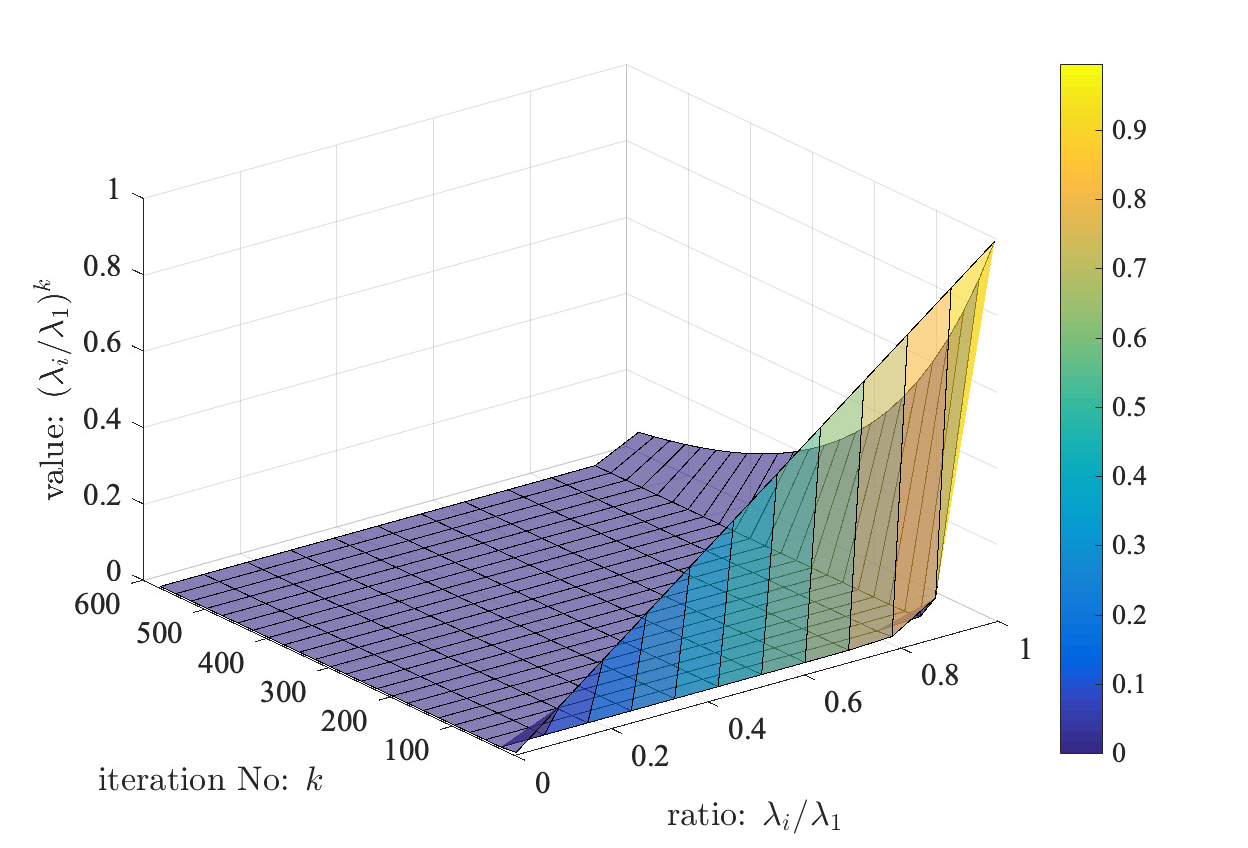
\includegraphics[width=0.7\linewidth]{curve.pdf}
\end{center}
\caption{Eigenvalue Ratio VS Number of Iterations.}
\label{fig: curve}
\end{figure}

Fig. \ref{fig: curve} shows how the value of $(\lambda_i/\lambda_1)^k$ evolves with different power iteration number $k$ and ratio~$\lambda_i/\lambda_1$. We need to select appropriate $k$ for different $\lambda_i/\lambda_1$ given $(0 < \lambda_i/\lambda_1 \leq 1)$. 

Let's assume $(\lambda_i/\lambda_1)^k<0.05$ being a good approximation to $(\lambda_i/\lambda_1)^k=0$. Then we have
\begin{equation}
(\lambda_i/\lambda_1)^k<0.05 \Leftrightarrow k\; \text{ln}(\lambda_i/\lambda_1) < \text{ln}(0.05) \Leftrightarrow k \geq \frac{\text{ln}(0.05)}{\text{ln}(\lambda_i/\lambda_1)}.
\end{equation}
The minimum value of $k$ to satisfy $(\lambda_i/\lambda_1)^k<0.05$ is $k = \lceil \frac{\text{ln}(0.05)}{\text{ln}(\lambda_i/\lambda_1)} \rceil$.

\begin{table}[!htb]
\begin{center}
\begin{tabular}{ccccccccccc}
\hline
$\lambda_i/\lambda_1$ & 0.2 & 0.4 & 0.6 & 0.8 & \textbf{0.85} & 0.9 & 0.95 & 0.99 & 0.995 & 0.999 \\ \hline
$k = \lceil \frac{\text{ln}(0.01)}{\text{ln}(\lambda_i/\lambda_1)} \rceil $     & 2   & 4   & 6   & 14  & \textbf{19}   & 29  & 59   & 299  & 598   & 2995  \\ \hline
\end{tabular}
\caption{The minimum value of $k$ we need to guarantee $(\lambda_i/\lambda_1)^k<0.05$.}
\label{tab: kmin}
\end{center}
\end{table}

Table \ref{tab: kmin} shows the minimum number of iterations we need to guarantee that the assumption holds. We can observe that when the two eigenvalues are very close to each other \emph{e.g.}, $\lambda_i/\lambda_1=0.999$, we need about 3000 iterations to achieve a good approximation. However, in practice, the case is very rare, and we set power iteration number to be 19. This will satisfy most of the cases. Besides, two very close eigenvalues usually leads to overflow according to Eq.\ref{eq: final-form} as the denominator $\lambda_1 - \lambda_i$ would be close to 0, but with our approximation, this problem could be avoided, and our method is more numerical stable.


\medskip
\small
\bibliographystyle{unsrt}
\bibliography{neurips_2019.bib}

\end{document}
